\documentclass{standalone}
\usepackage{tikz}
\usetikzlibrary{shapes}

\usepackage[T1]{fontenc}
\usepackage[utf8]{inputenc}
\usepackage{libertine}

\begin{document}
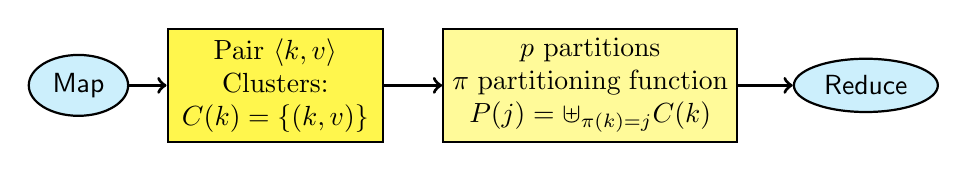
\begin{tikzpicture}[every node/.style={thick}]
  \colorlet{coul0}{orange!20} \colorlet{coul1}{blue!20} \colorlet{coul2}{red!20} \colorlet{coul3}{green!20}
  \tikzstyle{edge}=[->, very thick]
  \foreach \i in {1} {
    \node[ellipse, draw, fill=cyan!20] (map\i) at (3.5, 1.5 - \i) {\textsf{Map}};
  }
 {\textbf{Result}};
  \foreach \i in {1} {
    \node[draw, fill=yellow!70] (paire\i) at (6.0, 1.5 - \i) {\begin{minipage}{2.5cm}Pair \centering $\langle k,v \rangle$ \centering \\ Clusters: \\ $C(k) = \lbrace (k, v) \rbrace$ \end{minipage}};
    \node[draw, fill=yellow!40] (part\i) at (10.0, 1.5 - \i) {\begin{minipage}{3.5cm} \centering $p$ partitions \\ $\pi$ partitioning function \\ $P(j) = \uplus_{\pi(k) = j} C(k)$ \centering \end{minipage}};
    \node[ellipse, draw, fill=cyan!20] (reduce\i) at (13.5, 1.5 - \i) {\textsf{Reduce}};
    \draw[edge] (paire\i) -- (part\i);
    \draw[edge] (part\i) -- (reduce\i);
  }
          %paire
  \draw[edge] (map1.east) -- (paire1.west);
\end{tikzpicture}
\end{document}